\documentclass[notheorems]{beamer}
\usetheme{Warsaw}

\setbeamercovered{transparent}

\usepackage{amsmath, amssymb}
\usepackage{physics}

\theoremstyle{definition}
\newtheorem{definition}{Definition}

\author{Eli Griffiths}
\title{A Spectral Approach To Meshes}

\begin{document}

\begin{frame}
    \titlepage
\end{frame}

\begin{frame}
    \begin{columns}
    \begin{column}{0.5\pagewidth}
        \begin{definition}[Triangular Mesh]
            A \textbf{triangular mesh} is a triple $K = (V, E, F)$ such that
            \begin{itemize}
                \item<2-> $V \subseteq \mathbb{R}^3$ is a finite set representing the vertices
                \item<3-> $E \subseteq [V]^2$ is a set representing non-intersecting edges
                \item<4-> $F \subseteq [E]^3$ is the set of faces such that for any $f = \qty{e_1, e_2, e_3} \in F$, 
                    \begin{align*}
                        e_1 \cap e_2 &= \qty{v_1} \\
                        e_2 \cap e_3 &= \qty{v_2} \\
                        e_3 \cap e_1 &= \qty{v_3}
                    \end{align*}
                    for $v_1 \neq v_2 \neq v_3$. 
            \end{itemize}
        \end{definition}
    \end{column}

    \begin{column}{0.3\pagewidth}
        \begin{figure}
            \centering
            \only<1>{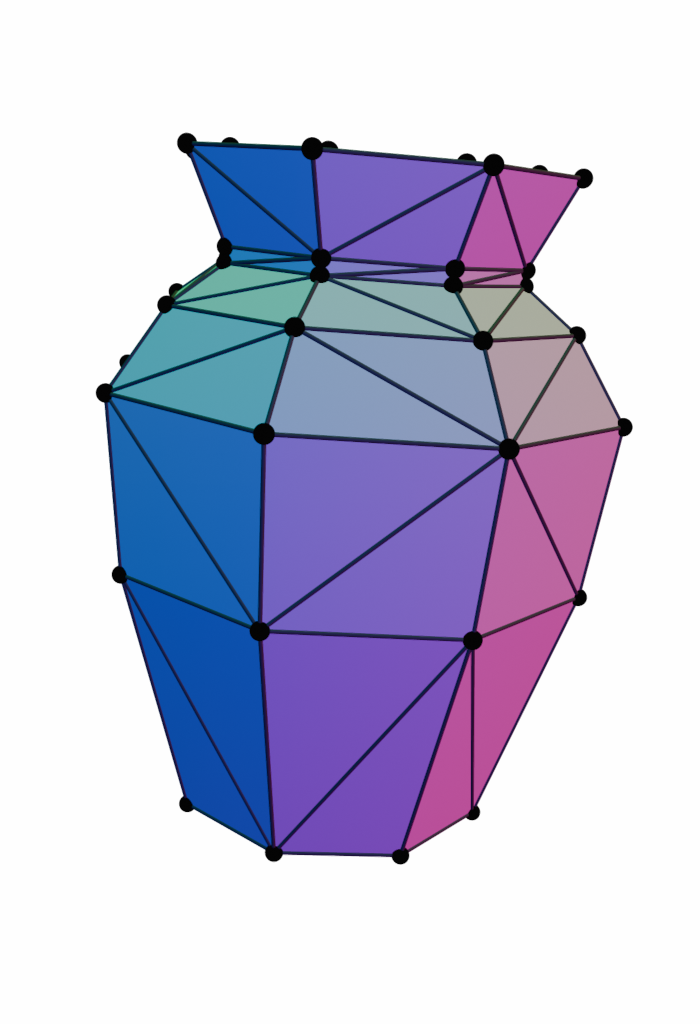
\includegraphics[width=0.3\pagewidth]{../figures/vase_all.png}}
            \only<2>{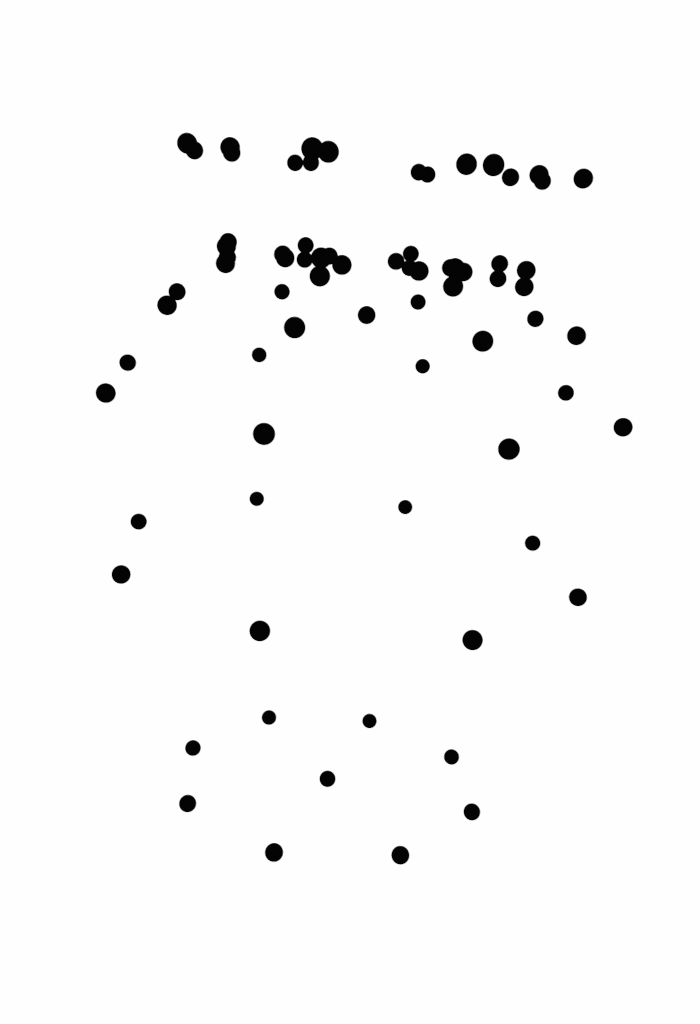
\includegraphics[width=0.3\pagewidth]{../figures/vase_vertices.png}}
            \only<3>{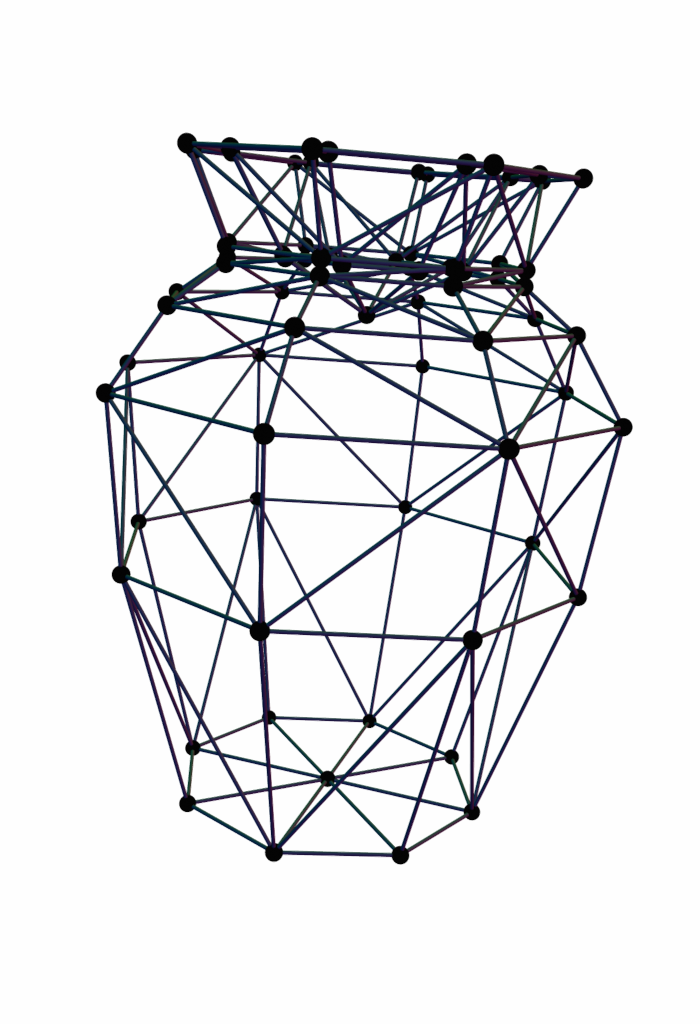
\includegraphics[width=0.3\pagewidth]{../figures/vase_edges.png}}
            \only<4>{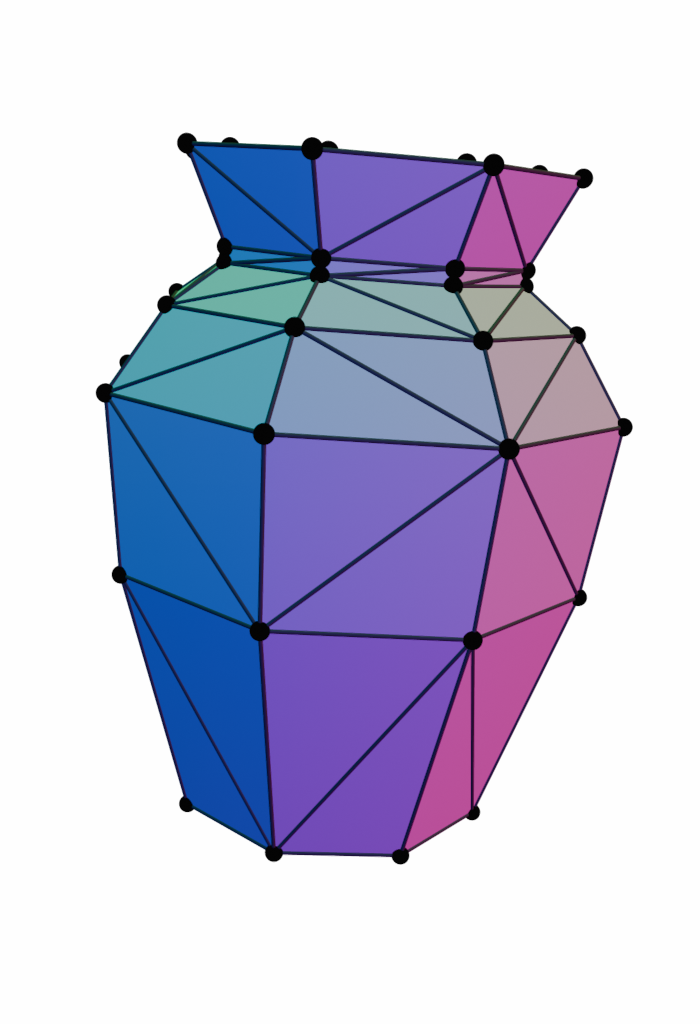
\includegraphics[width=0.3\pagewidth]{../figures/vase_all.png}}
        \end{figure}
    \end{column}
    \end{columns}
\end{frame}
    
\end{document}
